%----------------------------------------------------------------------------
\chapter{TPSC – Timed Property Sequence Charts}
%----------------------------------------------------------------------------
A TPSC[2] a PSC-nek egy kiterjesztése.
A PSC üzenetekre időzítési feltételeket specifikálhatunk.

\begin{figure}[!ht]
    \centering
    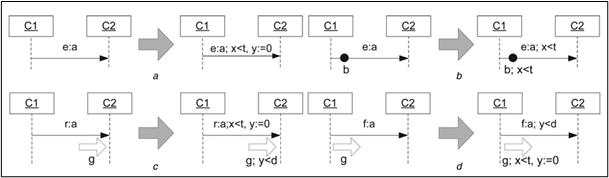
\includegraphics[width=150mm, keepaspectratio]{figures/4abra.png}
    \caption{PSC kiterjesztése időzítési feltételekkel[2].}
\end{figure}

A TPSC óraváltozókat (x, y) használ az időzítéshez.
Ezekre meg lehet adni feltételeket, valamint az óraváltozót lehet nullázni.
A nullázással adott eseménytől (pl. üzenet vételétől) kezdve indul az időzítés, majd rákövetkező események időbeliségét ez alapján lehet ellenőrizni.

A 3.1. ábrán látható, hogy például az \textit{e: a} sima üzenet \textit{e: a; x < t, y := 0} üzenetre bővül.
Elvárjuk, hogy az \textit{a} üzenet \textit{t} idő előtt történjen meg és egy \textit{y} óraváltozót nullázunk.
Az \textit{e: a} üzenet egy sima üzenet, szóval ha nem történik meg a specifikált idő intervallumban az nem jelent hibát.
Viszont \textit{r: a} üzenetnél már elvárt, hogy \textit{t} időn belül megtörténjen. \textit{f: a} üzenet esetében viszont akkor jelez hibát a monitor, ha üzenet megtörtént \textit{t} időn belül.

Egy megkötésre is meg lehet adni időzítési feltételt.
Így megadhatjuk, hogy mennyi ideig nem szabad jönnie a megkötésben szereplő nem kivánt üzenetek egyikének.
Ha a feltételben megadott idő után történik akkor az nem jelent hibát a monitor szempontjából.